\documentclass[12pt, oneside]{report}   	% use "amsart" instead of "article" for AMSLaTeX format
\usepackage{geometry}                		% See geometry.pdf to learn the layout options. There are lots.
\geometry{a4paper}                   		% ... or a4paper or a5paper or ... 
%\geometry{landscape}                		% Activate for for rotated page geometry
%\usepackage[parfill]{parskip}    		% Activate to begin paragraphs with an empty line rather than an indent
\usepackage{graphicx}				% Use pdf, png, jpg, or eps§ with pdflatex; use eps in DVI mode
\usepackage{float}					% TeX will automatically convert eps --> pdf in pdflatex

\usepackage{amssymb}
\usepackage{amsmath}
\usepackage[utf8]{inputenc}
\usepackage[german]{babel}
\usepackage[T1]{fontenc} % ermöglicht die Silbentrennung von Wörtern mit Umlauten
\usepackage[bookmarksnumbered, bookmarksopen=true]{hyperref}  % PDF wird mit Lesezeichen (verlinktes Inhaltsverzeichnis) versehen 

\usepackage{listings} 
%\usepackage{fancyhdr}
%\pagestyle{fancy}

%\fancyhead{}
%\fancyfoot{}

%\interfootnotelinepenalty=10000

\title{Twitter Sentiment Analyse}
\author{Jérémie Blaser, Nicolas Roos\\
	ZHAW (Zürcher Hochschule für Angewandte Wissenschaften),\\
	Zürich,\\
	Switzerland,\\
	\texttt{blaseje1@students.zhaw.ch},
	\texttt{roosnic1@students.zhaw.ch}}
\date{\today}							% Activate to display a given date or no date


%\fancyhead[C] {End-2-End Services/Monitoring}
%\fancyfoot[C] {Seite \thepage}
%\fancyfoot[L] {Nicolas Roos}
%\fancyfoot[R] {\today}


\begin{document}
\lstset{language=Python} 
\newcommand{\qem}[1]{\emph{"<#1">}} % quotated emphasize

\maketitle


%\paragraph{Ansprechpartner an der ZHAW} ~\\
%\begin{itemize}
%\item Studiengangleiter: Olaf Stern, Tel: +41 58 934 82 51; olaf.stern@zhaw.ch
%\end{itemize}


\tableofcontents



\chapter{Einleitung}
\section{Motivation}
Mit einer Sentiment Analyse über einen gewissen Zeitraum lässt sich zeigen was die Twitter Community von einem Brand, einer Firma, Personen usw. haltet. Diese Daten könnten Grafisch dargestellt werden und mit dem Aktienkurs der Firma oder signifikanten Ereignissen zu einem gewissen Zeitpunkt verglichen werden. 
\section{Idee}
Mit Suchwörtern wird nach allen Tweets gesucht welche zu einem bestimmten Thema/Firma/Hashtag gehören. Diese Tweets werden mit einer Sentiment Analyse Positiv oder Negativ eingestuft. Diese Einstufung wird in einem Zeit/Polarität Graph dargestellt. \\
Für diese Idee wird eine grosse Menge von Tweets über einen längeren Zeitraum (minimum 2 Monate) benötigt. Momentan ist noch nicht klar ob diese Menge vorhanden ist. Alternativ kann man auch die aktuellen Tweets nach Brand/Firma/Person filtern und über diese Tweets eine Sentiment Analyse laufen lassen.
\section{Meilensteine}
\begin{itemize}
\item Twitter-API anbinden/implementieren
\item Historische Sammlung von Tweets besorgen
\item Evaluation von MapReduce und MPI für unser Problem
\item Paralleles filtern von Tweets nach Keyword/Hashtag implementieren
\item Sentiment Analysis mit NLTK Classifier implementieren (Naive Bayes und MaxEnt)
\item Classifier Trainieren
\item Performanceanalyse erstellen
\item Vergleich Naive Bayes mit MaxEnt
\item GUI programmieren mit Plot des Stimmungsverlaufs
\item Dokumentation schreiben (Seminararbeit)
\end{itemize}


\chapter{Anforderungen}

\section{Twitter Korpus}
genügend Tweets um Klassifizierer zu trainieren, historischer verlauf
Twitter stellt für Entwickler eine moderne API (Application Programm Interface) zur Verfügung. Die aktuell version dieser API (Version 1.1) erlaubt dem Benutzer nach Tweets zu suchen oder die Timeline eines Benutzers anzuschauen. Die Menge von Tweets die bei solch einer Suche zurückgegeben wird, ist jedoch stark begrenzt. Pro Suche können ca. 15 Seiten mit maximal 100 Tweets gefunden werden\footnote{GET search. https://dev.twitter.com/docs/api/1/get/search. Zuletzt aufgerufen am 14.06.2014.}. Bei durchschnittlich 5700 Tweets pro Sekunde\footnote{New Tweets per second record, and how. https://blog.twitter.com/2013/new-tweets-per-second-record-and-how. Zuletzt aufgerufen am 14.06.2014} ist diese eine sehr geringe Menge. Dieser durchschnitt bezieht sich auf das Jahr 2013 und wird im Jahr 2014 sicherlich steigen.
Dadurch ist die Beschaffung von einer grossen Menge Tweets über die API nicht möglich. Als alternative gibt es Twitter Korpusse welche eine grosse Menge an Tweets beinhalten. 
\newline{}
Auf der Suche nach einem geeigneten Twitter korpus, für unsere Sentiment Analyse, wurden wir fündig auf www.sentiment140.com. Die Entwickler von sentiment140 haben eine Twitter Sentiment Analyse erfolgreich entwickelt und stellen ein Teil ihrer Testdaten zur Verfügung. Der Korpus beinhaltet 1,6 Millionen Tweets in einer CSV Datei und hat folgende 6 Datenfelder:
\begin{enumerate}
\item Polarität (0 = negativ, 2 = neutral, 4 = positiv)
\item ID des Tweets
\item Datum
\item Die Suchabfrage mit der der Tweet gefunden wurde
\item Benutzer welcher der Tweet geschrieben hat
\item Text des Tweets
\end{enumerate}
Obwohl wir unsere eigene Sentiment Analyse implementieren benötigen wir die Polarität, weil dadurch unsere eigener Klassifizierungs Algorithmen trainiert werden. Mehr dazu weiter unten. 

\section{Paralleles Rechnen}
Für die Parallellisierung wurde ein Python Framework benutzt. Für die Sentiment Analyse wird kein Cluster verwendet sondern mehrere Worker Prozesse welche auf dem Rechner parallel ausgeführt werden. Ein Grund dafür war dass die Klassifizierungs Algorithmen trainiert werden müssen um zu funktionieren. Diese Trainingsdaten über das Netzwerk auszurauschen, würden in unserem Fall zu einer Verlangsamung führen. %Mehr???
Zur Auswahl standen 2 Python Bibliotheken. Zum einen das Disco Framwork mit dem Map Reduce verfahren. Zum andern das  MPI for Python Framework mit dem Message Passing Interface verfahren.

lokalitäts Prinzip Mapreduce params wird sterilisiert. kein klassifizieret angeben

worker müssen trainierten classifier deserialisieren $\Rightarrow$ besser nicht über netzwerk
\subsection{Evaluation MapReduce vs. MPI}
\subsubsection{Disco - MapReduce}
Disco ist ein leichtes, Open-Source Framework dass das Map Reduce Programmiermodell, welches ursprünglich von Google entwickelt wurde\footnote{\textsc{Dean}, Jeffrey und \textsc{Ghemawat}, Sanjay: MapReduce: Simplified Data Processing on Large Clusters. In: Sixth Symposium on Operating System Design and Implementation, San Francisco 2004.}, anbietet. Für die Installation wird eine Linux/Unix Distribution oder ein Mac OS X System, einen SSH Daemon und Client, Erlang/OTP R14A oder neuer und Python 2.6.6 oder neuer benötigt. Für die Webdarstellung wird entweder Lighttpd 1.4.17 oder neuer oder Varnish 2.1.3 oder neuer benötigt. Disco kann auf dem Mac OS X mit Homebrew\footnote{Packet Manager für Mac OS X} installiert werden. Alternativ kann man auch den Source Code herunterladen und Disco selbständig kompilieren. Nach der installation braucht es noch einige kleinere Konfiguration bis Disco funktionsfähig ist. Ab jetzt kann mit Eingabedateien (Textdateien, CSV Dateien) und 2 Funktionen, Map und Reduce, das Framework benutz werden.
\subsubsection{MPI for Python - Message Passing Interface}
Das Message Passing Interface (MPI) ist ein Standard, welcher den Nachrichtenaustausch bei parallelen Berechnungen auf verteilten Computersystem beschreibt. Das MPI for Python Packte wurde auf den MPI-1/MPI2 Spezifikationen aufgebaut und bietet eine Objekt orientierte Schnittstelle an. Für die Installation von MPI for Python wird eine funktionierende MPI Distribution benötigt und Python 2.3 oder neuer. Die Installation ist relative einfach mit PIP\footnote{Installationsprogramm für Python-Pakete} auszuführen. Im Python Script wird die MPI Bibliothek importiert und die Scrips werden mit
\begin{lstlisting}
$ mpirun -n 5 python demo/helloworld.py
\end{lstlisting}
gestartet.\newline{}
%Noch nicht sicher ob das hierher gehört.
Wir haben uns für das Disco Framework entscheiden wegen der sehr einfachen Handhabung. Bei der Implementation der parallelen Sentiment Analyse haben wir jedoch bemerkt dass das Disco Framework Probleme hat beim Serialisieren und Deserialisieren des Klassifizierungsalgorithmus. Daher haben wir für die parallelisierung des Sentiment Analyse das MPI Framework verwendet.

\chapter{Umsetzung}

\section{Sentiment Analyse}
Die Sentiment Analyse ist ein Verfahren des \emph{Natural Language Processing}, einem interdisziplinären Forschungsgebiet aus Informatik und Linguistik.
Es geht im wesentlichen darum, die in einem Text vorherrschende Stimmung automatisiert zu bestimmen. 
Der zu untersuchende Text kann, wie in unserem Fall mit Tweets, aus nur einzelnen wenigen Sätzen bestehen, welche einer der beiden Klassen mit eher "<positiver"> oder "<negativer"> Stimmung zugeteilt werden.
Dafür verwendet man einen geeigneten Klassifikator, welchen  mit einer Trainingsmenge trainiert wird, um anschliessend die Klassifikation durchzuführen. 

Wir verwenden für diese Arbeit einen Naive-Bayes-Klassifikator sowie einen Maximum-Entropy-Klassifikator, zwei bekannte Klassifikationsalgorithmen des \emph{Machine Learning}, und vergleichen deren Leistung.


\subsection{Trainingsmenge}
Das Trainings-Set ist nach dem \emph{Bag of words model} aufgebaut.

\subsection{Klassifikationsalgorithmen}
\subsubsection{Naive-Bayes}

Der Naive-Bayes-Klassifikator macht sich die Wahrschentlichkeitsverteilung der Klassen und Features im Trainings-Set, sowie die Anwendung des Bayes-Theorem (Satz von Bayes) zunutze.
$$ P(C \mid F_1,\dots,F_n)$$

Satz von Bayes
$$
P(C \mid F_1,\dots,F_n) = \frac{P(C) \ P(F_1,\dots,F_n\mid C )}{P(F_1,\dots,F_n)}. \,
$$

$$ P(X,Y \mid Z) = P(X \mid Z) \ P(Y \mid Z) $$

naive, unabhängig -> bedingten unabhängigkeit
$$
P(C \mid F_1,\dots,F_n) = \frac{1}{W} \, P(C) \prod_{i=1}^n P(F_i\mid C)\ \ \ \mathrm{mit} \ \ W = P(F_1,\dots,F_n)
$$

$W$ konstant für aufruf -> weglassen
$$ \mathrm{classify}(f_1,\dots,f_n) = \underset{c \, \in \, \{pos,neg\} }{\operatorname{arg\,max}} \ P(c) \displaystyle\prod_{i=1}^n P(f_i\mid c) $$

die naive annahme entspricht nicht der realität, in der praxis jedoch gut ?cite?

In unserer Implementation verwenden wir die Klasse\\
 \verb|nltk.classify.NaiveBayesClassifier| des NLTK-Frameworks
 
%O(n)

\subsubsection{MaxEnt}
In unserer Implementation verwenden wir die Klasse\\
\verb|nltk.classify.scikitlearn.SklearnClassifier| zusammen mit\\
\verb|sklearn.linear_model.LogisticRegression| des scikit-learn Frameworks.

\subsection{Tweet Preprocessing}
@User, Hashtags, URLs, Retweets (RT), html entities
nltk-tokenizer

\section{Filtern mit MapReduce}

\section{Parallele Sentiment Analyse}

\section{GUI}


\chapter{Resultat}

\section{Naive Bayes vs. MaxEnt}

\begin{figure}[htbp]
\begin{center}
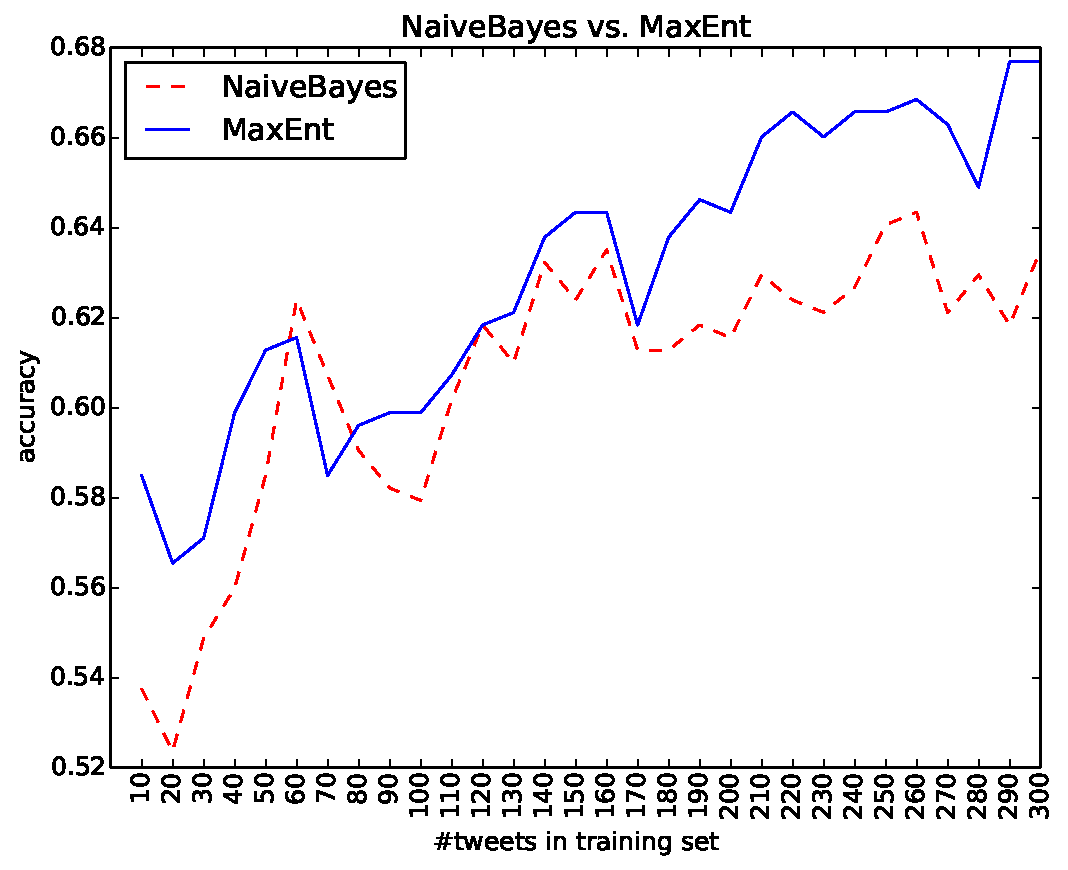
\includegraphics[width=0.9\textwidth]{bilder/cmp_nb_vs_me_S10_M300-16M.pdf}
\caption{Accuracy}
\label{img:acc}
\end{center}
\end{figure}

\begin{figure}[htbp]
\begin{center}
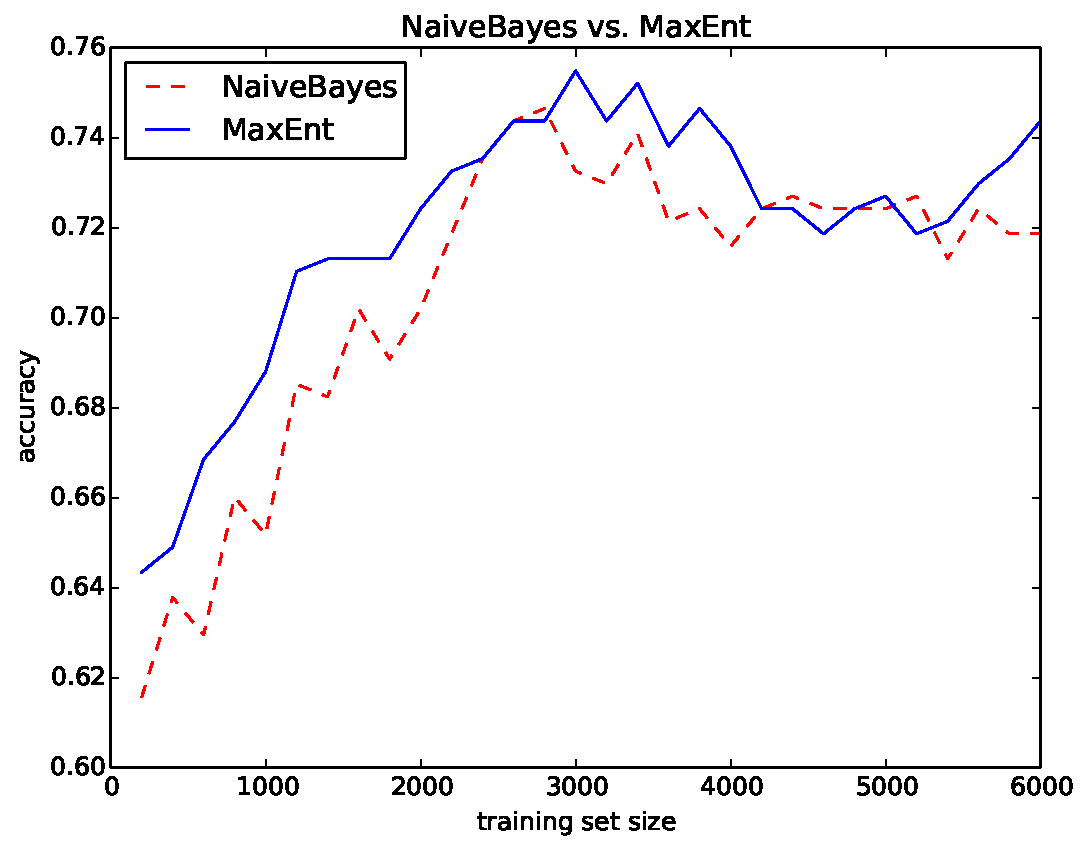
\includegraphics[width=0.75\textwidth]{bilder/cmp_nb_vs_me_S200_M6000.pdf}
\caption{Accuracy, Step 200}
\label{img:acc2}
\end{center}
\end{figure}

\begin{figure}[htbp]
\begin{center}
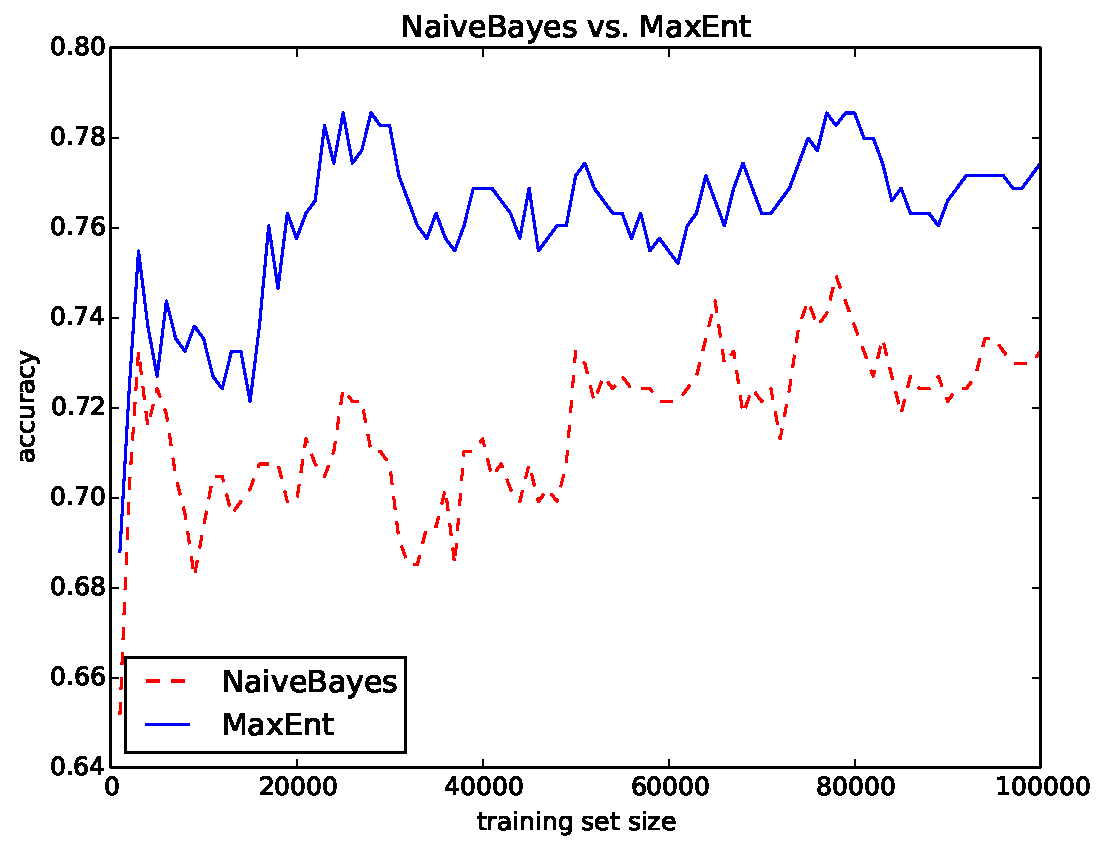
\includegraphics[width=0.75\textwidth]{bilder/cmp_nb_vs_me_S1000_M100000.pdf}
\caption{Accuracy, Step 1000}
\label{img:acc3}
\end{center}
\end{figure}


\section{Performancevergleich}

\begin{figure}[htbp]
\begin{center}
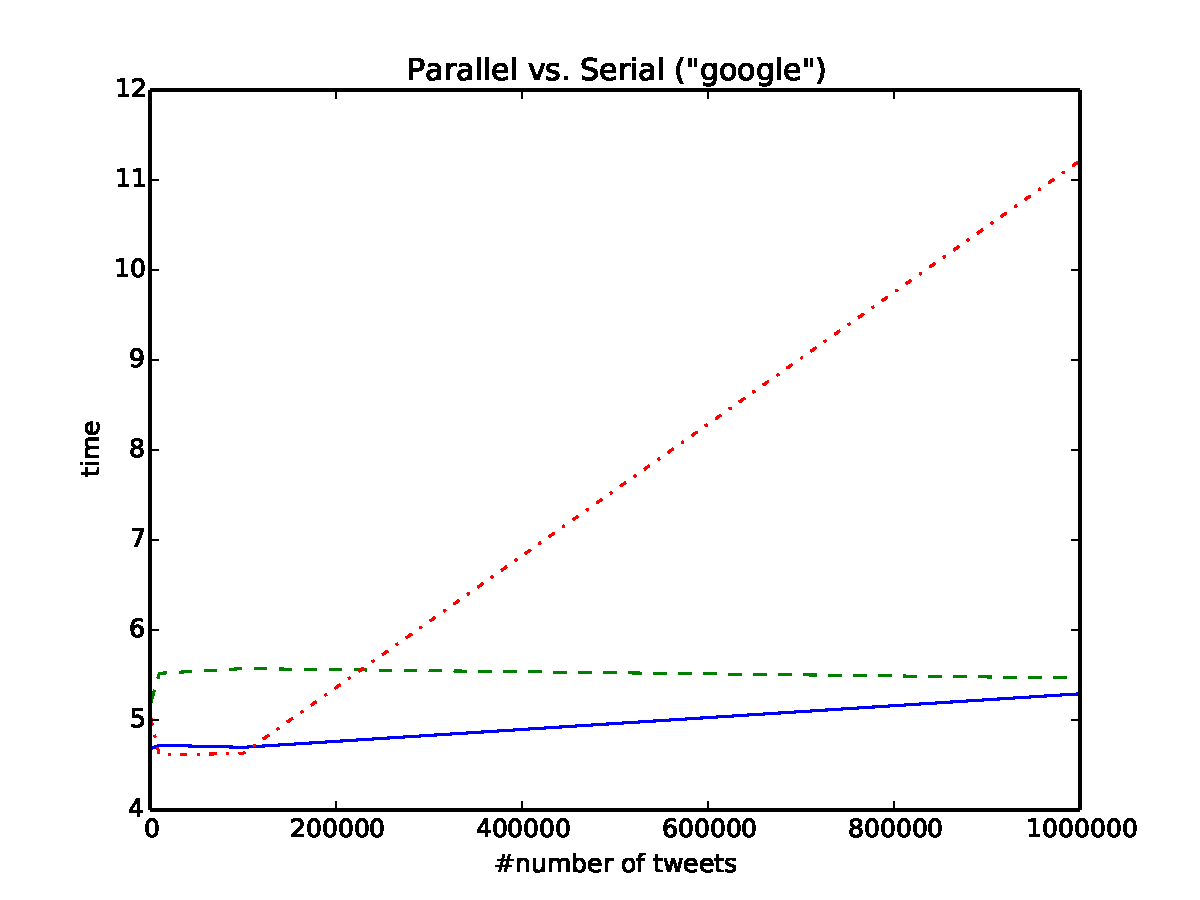
\includegraphics[width=0.9\textwidth]{bilder/time_par_vs_ser_google.pdf}
\caption{Performance}
\label{img:keyword 'google'}
\end{center}
\end{figure}

\begin{figure}[htbp]
\begin{center}
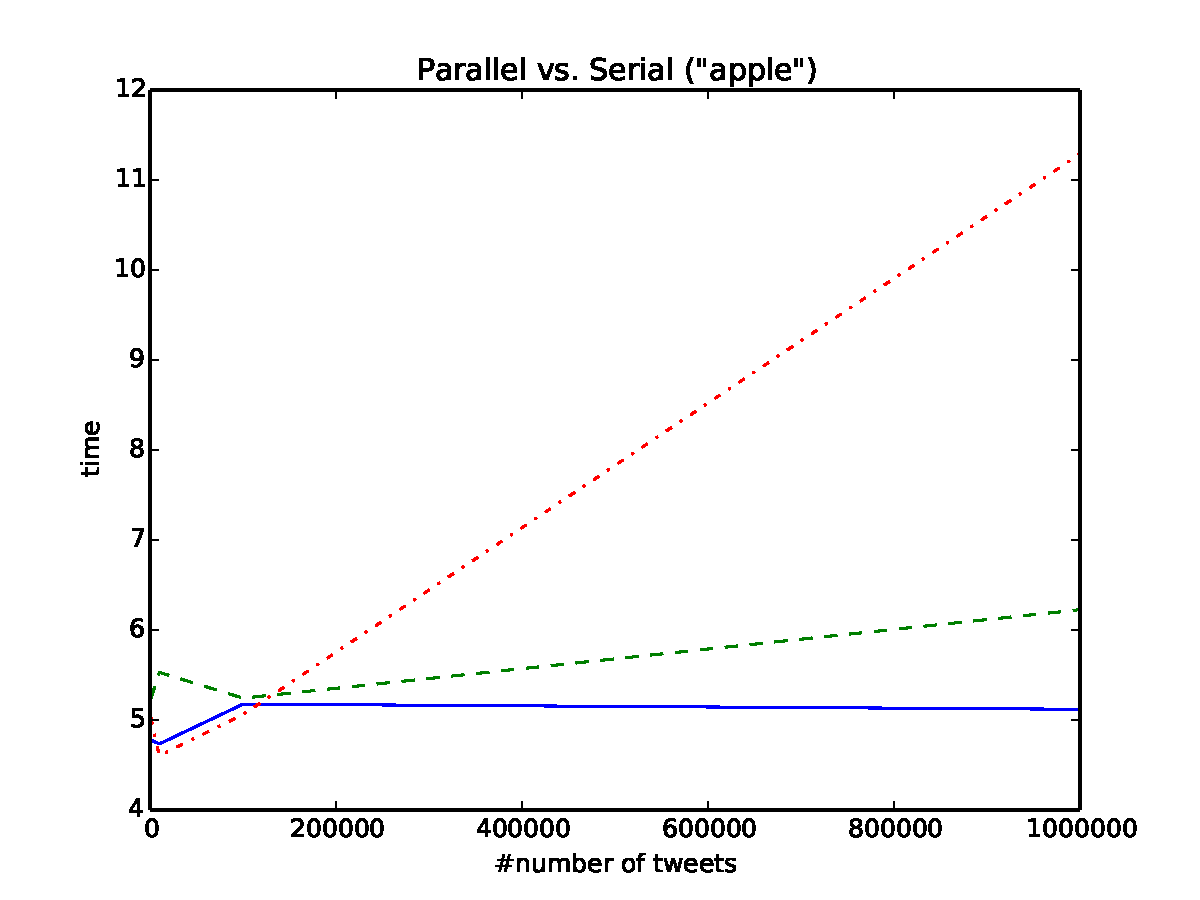
\includegraphics[width=0.9\textwidth]{bilder/time_par_vs_ser_apple.pdf}
\caption{Performance}
\label{img:keyword 'apple'}
\end{center}
\end{figure}

\section{Plot Stimmungsverlauf}


\chapter{Fazit}

\end{document}